\documentclass[tikz,border=2mm]{standalone}

\usepackage[T1]{fontenc}
\usepackage[swedish,english]{babel}
\usepackage{amsmath}
\usepackage{tikz}
\usepackage{amssymb}
\usetikzlibrary{shadows}
\usetikzlibrary{arrows,positioning}
\usepackage{pgfplots}


\begin{document}

% THE PICTURE BEGINS HEY?!!!
\begin{tikzpicture}[scale=1]
\definecolor{myBlue}{RGB}{57,106,177}; % (r,g,b) = (57,106,177)
\definecolor{myBrown}{RGB}{148,139,61};% (r,g,b) = (148,139,61)
% ORANGE HEY?
\definecolor{myOrange}{RGB}{213,94,0}
\definecolor{myBlueish}{RGB}{0,158,115}

\node at (0,0) (A){$\;$};
\node at (-3.9,1)
    {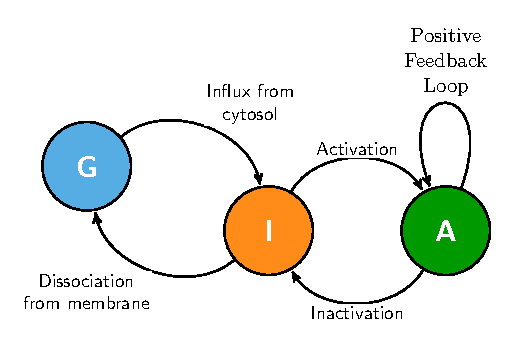
\includegraphics[scale=1.0]{activatorInhibitor.pdf}}; 
\node  at (3.7,1.3)
    {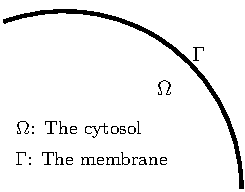
\includegraphics[scale=1.0]{simplifiedDomain/simplifiedDomain.pdf}}; 
    
\node[inner sep=0pt,below=2 of A]
    {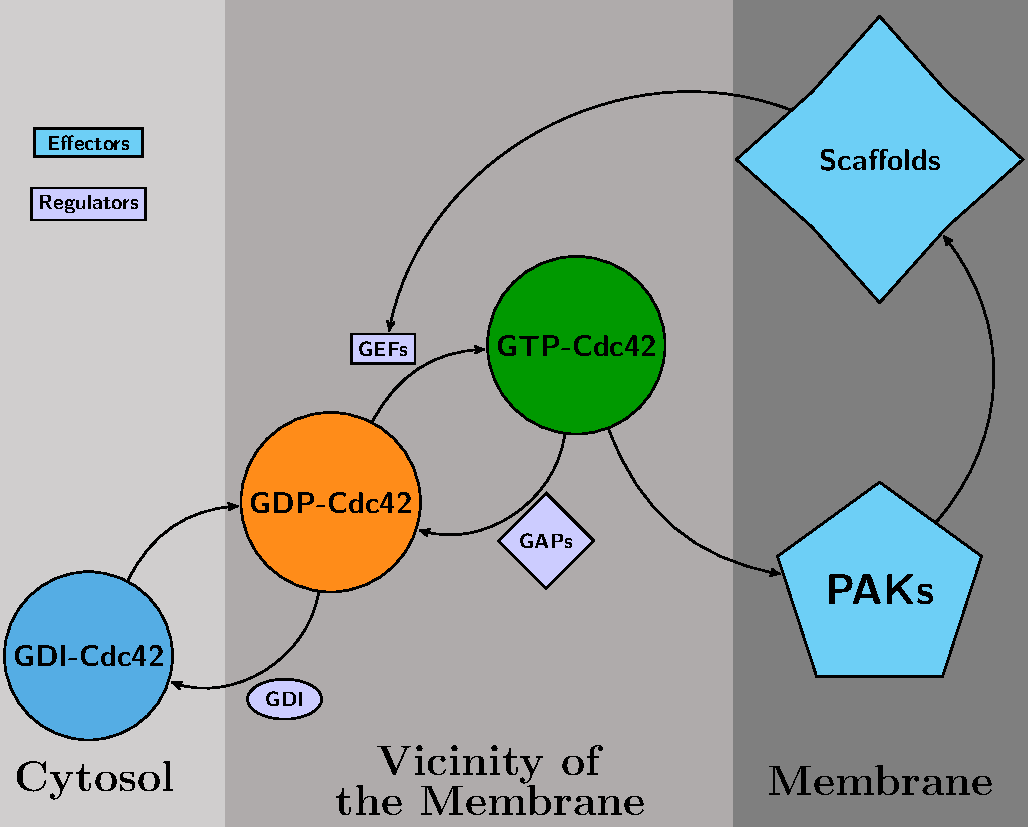
\includegraphics[scale=0.7]{reactionMechanism.pdf}};    
 
\node at (-7.5,3.5)(B) {\huge\textbf{(A)}};
\node[inner sep=0pt,right=7.5cm of B] {\huge\textbf{(B)}};
\node[inner sep=0pt,below=5cm of B] {\huge\textbf{(C)}};

\end{tikzpicture}








\end{document}
